\documentclass[aps,pra,twocolumn,reprint,floatfix,amsmath,amssymb]{revtex4-2}

\usepackage{graphicx}
\usepackage{booktabs}
\usepackage{siunitx}
\usepackage{hyperref}
\usepackage{array}

\begin{document}

\title{\texorpdfstring{Rigorous Echo-Ansatz Follow-Up for Shared-Line Multitone SQR in Dispersive cQED}{Rigorous Echo-Ansatz Follow-Up for Shared-Line Multitone SQR in Dispersive cQED}}
\author{Autonomous cQED Research Platform}
\affiliation{Shyam Shankar Quantum Circuits Group}
\date{\today}

\begin{abstract}
This follow-up revisits a narrow claim about selective qubit rotations in dispersive circuit quantum electrodynamics: whether the echoed sequence half-SQR \(\rightarrow \pi \rightarrow\) half-SQR \(\rightarrow \pi\) can rescue the strict simultaneous shared-line no-detuning multitone problem once the echo itself is treated as an optimizable ansatz rather than as a replay of a separately optimized half pulse. The underlying strict model is unchanged: one resonant tone per addressed manifold, no artificial per-tone detuning, and only per-tone amplitude and azimuth corrections. The earlier controlled no-go result still supplies the analytical baseline: spectator tones generate blockwise effective \(Z\) terms, and the stronger decoupled-block model succeeds only because it removes those spectators by assumption. The new contribution is a more careful echo study. We introduce a toggling-consistent echoed seed, allow independent corrections on the two active segments, compare against a total-duration-matched direct pulse, and report several phase-sensitive metrics rather than a single scalar fidelity. Across sixteen strict cases covering two Hamiltonian variants, two target families, addressed windows of size \(2\) and \(3\), and two durations, the plain direct shared-line pulse has mean restricted average gate fidelity \(0.7133\), while the exact reduced blockwise replay matches it to machine precision. A replayed ideal instantaneous echo drives the mean maximum residual-\(Z\) error down to \(9.78\times 10^{-3}\) rad, but its mean fidelity is only \(0.2006\) and its mean explicit probe-state fidelity is only \(0.0886\), demonstrating that a residual-\(Z\)-only metric can be badly misleading. Joint optimization of the ideal instantaneous echo raises the mean fidelity to \(0.5912\) and the best case to \(0.8098\); it outperforms the plain direct pulse in \(8/16\) cases, but only at the longer duration \(|\chi|T/2\pi=5\), and it never realizes the ideal gate. Once the refocusing pulses are made physical, the optimistic picture collapses. Two finite \(\SI{40}{ns}\) Gaussian \(\pi\) pulses give mean fidelity \(0.3176\) and never outperform the active-duration direct pulse. A manifold-aware shared-line multitone refocusing benchmark also fails to rescue the gate: the refocusing pulse itself has mean fidelity only \(0.1805\), and the echoed construction built from it reaches mean fidelity \(0.5073\) on the representative hard subset while remaining well below the plain direct baseline. The cautious verdict is therefore sharper than before: idealized echo can act as an upper bound and can modestly improve some long-duration special cases, but physical echoed multitone SQR does not rescue the strict no-detuning shared-line problem.
\end{abstract}

\maketitle

\section{Introduction}

The question in this report is deliberately narrower than generic gate synthesis in dispersive circuit quantum electrodynamics (cQED)~\cite{blais2004cavity,blais2021circuit,koch2007transmon}. We study selective qubit rotations implemented by one shared qubit-control line carrying one resonant tone per addressed cavity manifold. The strict control restriction is unchanged from the preceding no-go study: no artificial per-tone detuning is allowed, and the only free corrections are per-tone amplitude and azimuth.

The previous study established a controlled no-go statement for that strict problem and also tested two echoed constructions. The open loophole was not analytical but methodological: the negative echo result used inherited half-pulse replay rather than a genuine sequence-level echo optimization. This follow-up closes that loophole.

Three distinctions are essential.
\begin{enumerate}
  \item The controlled no-go remains a statement about the strict simultaneous shared-line problem, not about richer control families.
  \item The stronger decoupled-block approximation remains an exact counterexample only because it removes the shared-line spectator mechanism by assumption.
  \item Echo must be evaluated on phase-sensitive gate metrics, not only on a residual-\(Z\) surrogate, because an echo can reduce one error channel while still failing badly as a gate.
\end{enumerate}

\section{Model, Scope, and Metrics}
\label{sec:model}

We use the block-resolved dispersive Hamiltonian
\begin{equation}
H_0 = \sum_n \frac{\omega_n}{2}\sigma_z \otimes |n\rangle\langle n|,
\end{equation}
with manifold frequencies
\begin{equation}
\omega_n = \omega_q + \chi n + \chi' n(n-1) + \cdots .
\end{equation}
The shared-line multitone drive is
\begin{equation}
H_d(t)=\sum_{m\in \mathcal S}\frac{\Omega_m f(t)}{2}
\left[e^{-i(\omega_m t-\phi_m)}\sigma_+ + e^{i(\omega_m t-\phi_m)}\sigma_- \right],
\end{equation}
where each \(\omega_m\) is fixed exactly at the chosen block transition frequency. No independent \(Z\)-compensation or per-tone detuning term is allowed.

The target ideal selective rotation is
\begin{equation}
U_{\mathrm{SQR}}^{\mathrm{ideal}}=\bigoplus_{n\in\mathcal S}R_{\hat n(\varphi_n)}(\theta_n),
\end{equation}
with \(R_{\hat n(\varphi)}(\theta)\) a pure \(XY\)-plane rotation. Every addressed block must therefore end with no residual block-dependent \(Z\) phase.

The numerical grid is smaller than in the preceding report but deeper in the echo direction:
\begin{itemize}
  \item two Hamiltonian variants: \(\chi\)-only and \(\chi+\chi'\),
  \item two target families: aligned \(x\) and structured \(XY\),
  \item addressed windows \(N_{\mathrm{active}}=2,3\),
  \item two durations: \(|\chi|T/2\pi=3,5\),
  \item exact shared-line propagation through the local \texttt{cqed\_sim} stack~\cite{cqed_sim}.
\end{itemize}

Because the echo question is especially vulnerable to metric choice, we report several diagnostics rather than a single fidelity number. The most important are: the restricted process fidelity and restricted average gate fidelity on the addressed logical subspace; the best-fit restricted process fidelity after logical block-phase removal; the spanning-set state-transfer mean; the mean and minimum fidelities over an explicit probe set containing cavity superpositions and fixed random logical states; blockwise residual-\(Z\) and transverse error-generator components; and leakage into wrong addressed blocks or outside the addressed logical subspace altogether.

\section{Controlled No-Go Baseline}
\label{sec:nogo}

The analytical baseline is unchanged. In the interaction frame of \(H_0\), block \(n\) sees
\begin{equation}
H_I^{(n)}(t)=f(t)\sum_{m\in\mathcal S}\lambda_m X_{\phi_m-\Delta_{nm}t},
\end{equation}
with \(\lambda_m=\Omega_m/2\) and \(\Delta_{nm}=\omega_m-\omega_n\). The resonant term is static and transverse, while every spectator tone remains in the same block as an off-resonant transverse drive. For a square pulse, the second Magnus term produces a blockwise \(Z\) generator
\begin{equation}
\overline{H}_n^{(2)}=\zeta_n Z,
\end{equation}
and for two addressed blocks the coefficients take the explicit form
\begin{align}
\zeta_0 &= -\lambda_1^2 K(\Delta,T)+\lambda_0\lambda_1 L(\Delta,T,\delta), \\
\zeta_1 &= +\lambda_0^2 K(\Delta,T)-\lambda_0\lambda_1 L(\Delta,T,\delta),
\end{align}
with \(K(\Delta,T)>0\) for \(\Delta,T>0\). Canceling both \(\zeta_0\) and \(\zeta_1\) therefore requires nongeneric extra relations beyond the amplitude and azimuth choices already needed to match the target transverse rotations.

The present report keeps that result deliberately scoped: it is a controlled statement inside the dispersive block-resolved model, not an all-regime theorem for arbitrary strong driving. Numerical work is still needed to test whether exact shared-line propagation finds counterexamples. It does not.

\section{Strict Shared-Line Baselines}
\label{sec:baselines}

The direct strict shared-line pulse has mean restricted average gate fidelity \(0.7133\) across the sixteen cases, with best case \(0.8058\). The exact reduced blockwise replay matches the full shared-line result to machine precision: the minimum reduced-versus-full restricted process fidelity and restricted average gate fidelity are both \(1.0\). The failure is therefore already present in the block-resolved shared-line dynamics rather than being caused by leakage.

By contrast, the stronger decoupled-block approximation again realizes the ideal target exactly. Figure~\ref{fig:scaling} shows the contrast versus addressed-window size.

\begin{figure}[tb]
  \centering
  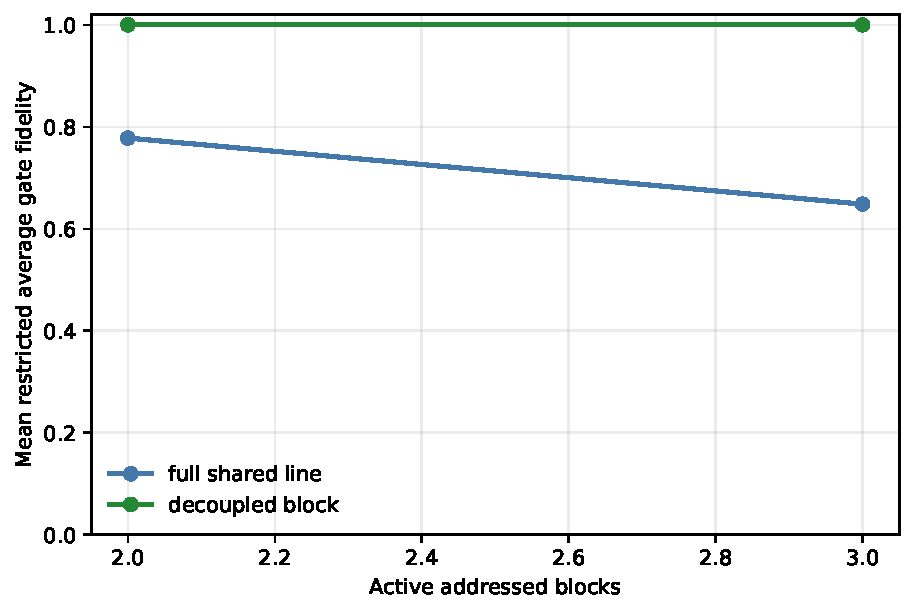
\includegraphics[width=\columnwidth]{../figures/addressed_subspace_scaling.pdf}
  \caption{Mean restricted average gate fidelity versus addressed-window size. The stronger decoupled-block approximation remains exact because it removes spectator tones by assumption; the physical simultaneous shared-line construction does not.}
  \label{fig:scaling}
\end{figure}

Figure~\ref{fig:duration} shows the duration tradeoff for the direct pulse, the total-duration-matched direct comparator, and the two main optimized echo variants. The matched direct pulse is important because any finite echo necessarily lasts longer than the plain active-duration pulse.

\begin{figure}[tb]
  \centering
  
\includegraphics[width=\columnwidth]{../figures/duration_fidelity_tradeoff.pdf}
  \caption{Median restricted average gate fidelity versus normalized active duration. The plain strict shared-line pulse is the main physical baseline. The total-duration-matched direct pulse is included only as a fairness comparator for finite echoes.}
  \label{fig:duration}
\end{figure}

\section{Echoed Ansatz Follow-Up}
\label{sec:echo}

\subsection{Ansatz and conventions}

The echoed sequence is
\begin{equation}
U_{\mathrm{echo}} = X_{\pi}\,U_2\,X_{\pi}\,U_1.
\end{equation}
Here \(U_1\) and \(U_2\) are the two active multitone segments and \(X_\pi\) is the refocusing pulse. This follow-up differs from the earlier echo test in two ways.
\begin{enumerate}
  \item The second active segment is seeded in the toggling-consistent way: if the target azimuth is \(\varphi_n\), the nominal second-half azimuth is \(-\varphi_n\) because \(X_\pi Y X_\pi=-Y\).
  \item The two active segments receive independent amplitude and azimuth corrections, and a weak duration-asymmetry parameter is optimized at the sequence level.
\end{enumerate}

We compare four echoed constructions:
\begin{enumerate}
  \item replayed ideal instantaneous echo,
  \item jointly optimized ideal instantaneous echo,
  \item jointly optimized finite Gaussian echo with two \(\SI{40}{ns}\) vacuum-calibrated \(\pi\) pulses,
  \item a representative subset with a separately optimized manifold-aware shared-line multitone refocusing pulse.
\end{enumerate}

\subsection{Why residual-\(Z\) alone is not enough}

The replayed ideal instantaneous echo is the clearest cautionary example. It drives the mean maximum residual-\(Z\) error down from \(9.36\times10^{-2}\) rad for the direct strict pulse to \(9.78\times10^{-3}\) rad. If one inspected only a residual-\(Z\) diagnostic, this could look like success. It is not. The same replayed construction has mean restricted average gate fidelity only \(0.2006\) and mean explicit probe-state fidelity only \(0.0886\). The echo removes one error channel while catastrophically failing the gate.

That observation matters because it explains why earlier or narrower echo analyses could look more positive than they were. A metric insensitive to the full logical action can hide the real failure mode.

\subsection{Optimized ideal instantaneous echo}

Once the echo is optimized as a genuine ansatz, the picture becomes subtler. The mean restricted average gate fidelity rises from \(0.2006\) for replayed ideal echo to \(0.5912\), and the best case reaches \(0.8098\). The optimized ideal instantaneous echo outperforms the plain strict direct pulse in \(8/16\) cases, but all eight of those improvements occur only at the longer duration \(|\chi|T/2\pi=5\). At the shorter duration \(|\chi|T/2\pi=3\), the optimized ideal echo never beats the direct pulse.

This is the correct interpretation of the idealized echo: it is a useful upper bound and can improve some long-duration special cases, but it is not an exact rescue. Its mean fidelity remains below the direct baseline (\(0.5912\) versus \(0.7133\)), and no case reaches the ideal gate.

\subsection{Finite Gaussian echo}

The physically relevant result is the finite-pulse echo. Here the verdict remains negative. The jointly optimized Gaussian echo has mean restricted average gate fidelity \(0.3176\), mean maximum residual-\(Z\) error \(0.4913\) rad, and mean probe-state fidelity \(0.4177\). It never outperforms the plain active-duration direct pulse. It does beat the total-duration-matched direct comparator in \(3/16\) cases, all of them structured-\(XY\) three-block cases, but those ``wins'' occur at poor absolute fidelity values between \(0.318\) and \(0.448\). That is not a rescued gate.

Figure~\ref{fig:echocompare} summarizes the family-averaged comparison, and Fig.~\ref{fig:tradeoff} shows the direct-matched tradeoff view.

\begin{figure}[tb]
  \centering
  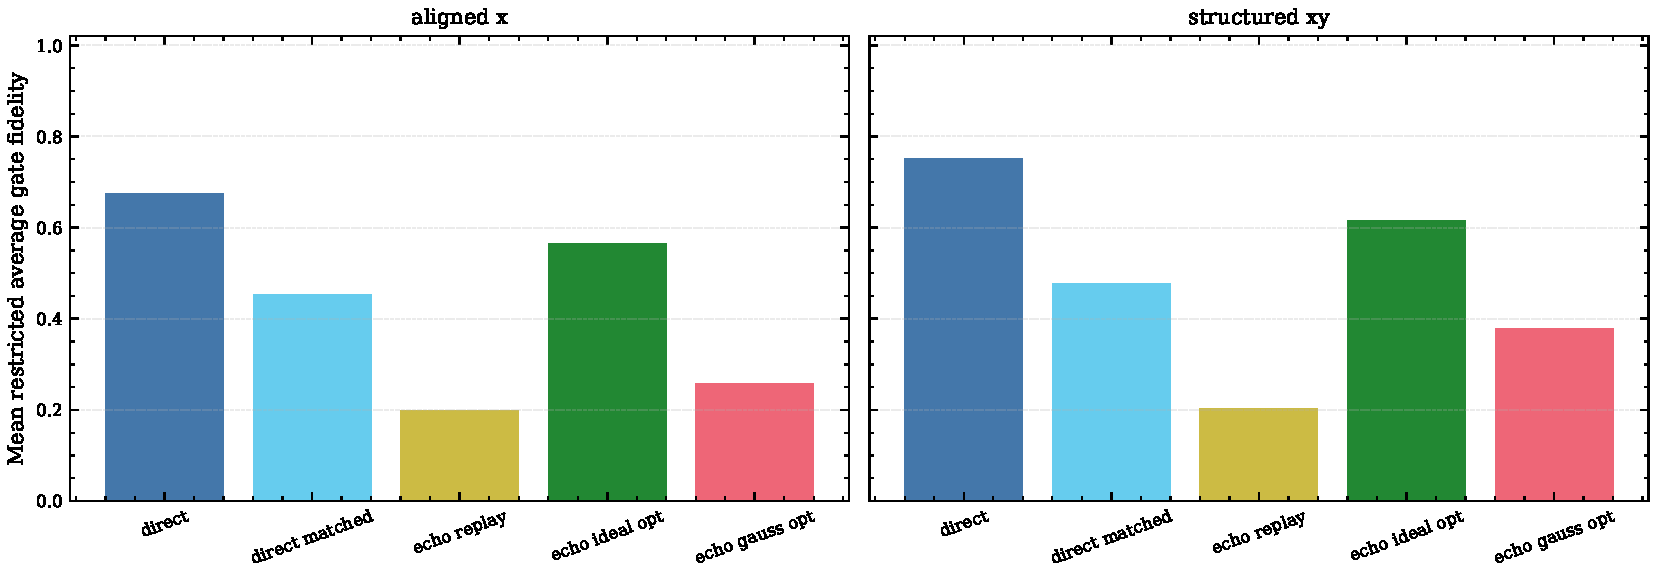
\includegraphics[width=\columnwidth]{../figures/plain_vs_echo_comparison.pdf}
  \caption{Family-averaged fidelity comparison. Sequence-level ideal echo optimization improves dramatically over naive replay, but the finite Gaussian echo remains far below the plain direct baseline.}
  \label{fig:echocompare}
\end{figure}

\begin{figure}[tb]
  \centering
  
\includegraphics[width=\columnwidth]{../figures/echo_delta_tradeoff.pdf}
  \caption{Finite-echo tradeoff versus the total-duration-matched direct comparator. Some finite echoes reduce residual-\(Z\) relative to the longer direct pulse, but not enough to deliver a practically good gate.}
  \label{fig:tradeoff}
\end{figure}

\subsection{Manifold-aware multitone refocusing}

One obvious future-work question from the earlier report was whether the negative finite-echo result was simply caused by the vacuum-calibrated Gaussian \(\pi\) pulse. We therefore tested a stronger alternative on the representative harder subset \((\chi+\chi')\) and \(|\chi|T/2\pi=5\): a shared-line multitone refocusing pulse optimized directly for blockwise \(R_x(\pi)\).

That benchmark does not rescue the gate. The refocusing pulse itself has mean restricted average fidelity only \(0.1805\), which already signals the problem: the same strict no-detuning shared-line resource is a poor way to realize a uniform blockwise \(X_\pi\) pulse. The echoed construction built from that refocusing pulse reaches mean fidelity \(0.5073\) on the four-case hard subset. This is better than the total-duration-matched direct comparator on that subset (\(0.4627\)) but still far below the plain direct pulse (\(0.7080\)), and its mean maximum residual-\(Z\) error is \(1.103\) rad. Figure~\ref{fig:refocus} shows the refocusing benchmark directly.

\begin{figure}[tb]
  \centering
  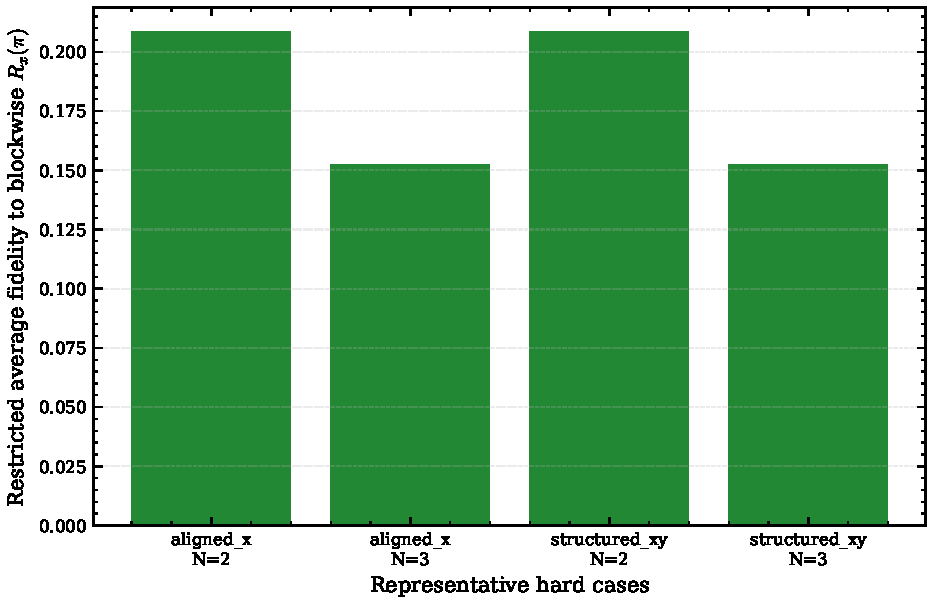
\includegraphics[width=\columnwidth]{../figures/refocus_multitone_pi_benchmark.pdf}
  \caption{Representative benchmark for the manifold-aware shared-line multitone refocusing pulse. The refocusing problem itself is already poorly solved under the strict no-detuning shared-line ansatz.}
  \label{fig:refocus}
\end{figure}

\section{Final Verdict}
\label{sec:verdict}

The updated answers are:

\paragraph*{1. Is exact ideal simultaneous shared-line multitone SQR possible under the physical no-detuning amplitude-plus-azimuth model?}
Not generically, and this follow-up found no exact counterexample. The best strict direct case remains about \(0.806\) restricted average gate fidelity, not unity.

\paragraph*{2. Under what assumptions is it impossible?}
Under the same controlled assumptions as before: the dispersive block-resolved shared-line model, tones fixed at the block transitions, no artificial detuning, and the ideal target defined as a direct sum of pure \(XY\) rotations with no block-dependent \(Z\) phase.

\paragraph*{3. Under what stronger approximation does ideal SQR become achievable?}
Under the stronger decoupled-block approximation that drops all spectator tones exactly in each block. That approximation changes the physical problem and must not be conflated with the simultaneous shared-line one.

\paragraph*{4. Does the echoed multitone sequence rescue the situation exactly, approximately, or only in special regimes?}
It does not rescue the physical gate. A replayed ideal echo can suppress residual \(Z\) while failing catastrophically on phase-sensitive gate metrics. A jointly optimized ideal instantaneous echo is a meaningful upper bound and can improve some long-duration special cases, but it is still not exact and does not win overall. Once the refocusing pulses are made physical, the echoed constructions remain far from the ideal gate.

\section{Limitations and Future Work}
\label{sec:limitations}

The strongest remaining caveat is conceptual rather than numerical. The ideal instantaneous echo is an upper-bound thought experiment, not a physical pulse sequence. This report therefore separates the exact mathematical question from the practical gate-design question. The practical verdict is based on the finite Gaussian and manifold-aware multitone refocusing studies, both of which remain poor.

The next useful extensions are now clearer than before.
\begin{itemize}
  \item Chart the lower-dimensional accidental near-cancellation set more explicitly, especially in the long-duration two-block regime where the idealized echo can modestly help.
  \item Study the minimum extra control resource that genuinely changes the physical verdict, such as per-tone detuning or explicit logical \(Z\)-compensation.
  \item Upstream the exact reduced replay and blockwise error-generator diagnostics into the local simulation framework, because they were essential for auditing the conclusions here.
\end{itemize}

\appendix

\section{Numerical Details and Validation}
\label{app:validation}

The production sweep contains sixteen main cases and four additional manifold-aware refocusing subset cases. The full run took about \(\SI{1810}{s}\) wall clock on the local workstation.

The direct strict and exact reduced blockwise-replay constructions agree to machine precision: the minimum reduced-versus-full restricted process fidelity and minimum reduced-versus-full restricted average gate fidelity are both \(1.0\). The decoupled-block construction again reproduces the ideal target exactly with unit fidelity.

The representative convergence case used for the follow-up validation is the \(\chi+\chi'\), aligned-\(x\), three-block, \(|\chi|T/2\pi=5\) instance. Increasing the direct optimization budget leaves the restricted average gate fidelity at \(0.5921\) within the reported digits, while the higher-budget finite Gaussian echo remains poor and does not approach the ideal gate.

\begin{table}[tb]
  \centering
  \scriptsize
  \caption{Aggregate construction means from the full follow-up sweep.}
  \label{tab:aggregate}
  \begin{tabular}{@{}lccc@{}}
    \toprule
    Construction & Count & Mean fidelity & Best fidelity \\
    \midrule
    Direct & 16 & 0.7133 & 0.8058 \\
    Direct, total matched & 16 & 0.4656 & 0.6130 \\
    Replay ideal echo & 16 & 0.2006 & 0.2054 \\
    Optimized ideal echo & 16 & 0.5912 & 0.8098 \\
    Optimized Gaussian echo & 16 & 0.3176 & 0.4575 \\
    Refocus benchmark & 4 & 0.1805 & 0.2085 \\
    Echo with multitone refocus & 4 & 0.5073 & 0.6591 \\
    \bottomrule
  \end{tabular}
\end{table}

\section{Reproducibility}
\label{app:repro}

The machine-readable outputs include the full result table, the metric definitions, the validation payload, and per-case artifacts with restricted operators, waveform samples, and probe-state diagnostics. The required reproducibility notebook rebuilds the principal figures and summary tables from those saved artifacts.

\bibliographystyle{apsrev4-2}
\bibliography{references}

\end{document}
